\chapter{From the projective Hilbert space to state manifolds}
\textit{\today\newline
Jan Střeleček\newline}

\section{Projective Hilbert space}
Consider the Hilbert space $\H$ to be a space of \emph{bare states} and $\mathcal{S}$ to be the space of \emph{normalized bare states}. Physical observables are related to the \emph{space of rays}, defined as $\PH\coloneqq \mathcal{H}/U(1)$, for the factorization by elements of $U(1)$. This group consists of unitary transformations $e^{i\phi}$ for $\phi\in\R$, defining gauge symmetry between quantum states. $\PH$ is then considered to be the \emph{space of pure states}. For the sake of generality, let's not normalize our vectors yet, which would lead to the \emph{space of unnormalized pure physical states}. 

It can be shown, that $\PH$ is of a K\"ahler structure, meaning it has two non-degenerate sesquilinear\footnote{We are in physics, so complex conjugated is the first input of the 2-form.} 2-forms embedded along with operator complex unit
$$(J, G, \Omega),$$
such that
\begin{equation}
    J^2=\Id
\end{equation}
and any bracket of $\ket{\psi_1},\ket{\psi_2}\in \PH$ can be decomposed into real and imaginary part\citep{ashtekar_geometrical_1997}
\begin{equation}
    \braket{\psi_1|\psi_2}=\frac{1}{2}G(\psi_1,\psi_2)-\frac{i}{2}\Omega(\psi_1,\psi_2).
    \label{eq:quantumProd}
\end{equation}

From braket sesquilinearity goes that $G$ is symmetric and $\Omega$ antisymmetric form, thus they can be uniquely written into one 2-form called \emph{Fubini-Study metric} with property
\begin{equation}
    G=\Re Q ;\qquad \Omega=\Im Q.
\end{equation}

Because $\braket{\psi_1|\psi_2}\in[0,1]$ we say, that the metric is measuring the geodesic distance on the Bloch sphere. Here if we define
\begin{equation}
    |\braket{\psi_1|\psi_2}|=\cos^2 \frac{\theta}{2},
\end{equation}
we get $\d \theta= 2\d s=2\sqrt{|g_{\mu\nu}\d \llambda^\mu\d \llambda^\nu|}$, see \citet{cheng_quantum_2013}.

To write the metric in a standard form, we need to realize how our space looks like. For finite $n+1$-dimensional Hilbert space, one dimension is lost in the gauge transformation, leaving us with $n$-dimensional $\PH$. Another dimension is lost due to normalization, which is usually done by mapping to an n-dimensional complex sphere
$$CP^n= \left\{ \Z=(Z_0,Z_1,\dots,Z_n)\in \mathbb{C}^{n+1}/\{0\} \right\}\Big/ \{\Z\sim c\Z \text{ for } c\in \mathbb{C}\}.$$

Natural property of such complex spaces is splitting of its tangent space to holonomous and anholonomous part\footnote{$T^{p,q}\M$ means $p+q$- cotravariant space (the space of vectors) on $\M$. The line over letter means complex conjugation.}
$$T^{1,0}\M=\Span\left\{\frac{\partial}{\partial Z_i}\right\}; \qquad T^{0,1}\M=\Span\left\{\frac{\partial}{\partial Z_{\overline{i}}}\right\}.$$


Distance on $\mathbb{C}^{n+1}$ is standardly defined using Hermitean metric\footnote{which is by definition sesquilinear, as one would expect in quantum mechanics later on} 
\begin{equation}
    \d s^2 = \d \overline{\Z} \otimes \d \Z.
\label{eq:metricdistancePH}
\end{equation}


For \emph{normalized states} in quantum mechanics is $\d Z=??????$, which plugged into Eq. \ref{eq:metricdistancePH} yields
\begin{equation}
    \d s^2 = 1-\left|\braket{\psi+\delta \psi|\psi}\right|^2.
    \label{eq:distanceInPH}
\end{equation}


\section{Restriction to eigenstate manifolds}
In quantum mechanics, one can examine a Hamiltonian $\HH(\llambda)$, for some parameter $\llambda\in \R^n$. At every point $\llambda$ we get projective Hilbert space $\PH(\llambda)$. This creates a fibre structure space, in which there are some section with interesting physical applications. Some of those sections are \emph{eigenstate manifolds}, defined by setting only one non-zero coefficient $Z_k$ in eigenbasis $\ket{\psi}=\sum_{k=0}^n Z_k \ket{k}$. From normalization goes automatically $Z_k=1$. The distance is then
\begin{equation}
    \begin{split}
        \d s^2 &= \textcolor{gray}{1}-\bra{k+\delta k}\textcolor{gray}{k\rangle \langle k}\ket{k+\delta k}=\textcolor{gray}{1}-\bra{k+\delta k}\textcolor{gray}{\big(\Id-\sum_{j\neq k} \ket{j}\bra{j}\big)}\ket{k+\delta k} \\
        &= \textcolor{gray}{\sum_{j\neq k}}\bra{k+\delta k}\textcolor{gray}{j\rangle \langle j}\ket{k+\delta k}.
        \label{eq:dsDerivation}
    \end{split}
\end{equation}
Using the \Schrodinger equation $\textcolor{blue}{\HH}\ket{k}=\textcolor{teal}{E_k} \ket{k}$, distributivity of derivative and projection to some state $\textcolor{gray}{\bra{j}}$, we get
\begin{equation}
    \begin{split}
        \textcolor{blue}{\HH}\ket{k} &= \textcolor{teal}{E_k}\ket{k}\\
        \textcolor{blue}{(\delta \HH)}\ket{k} +\textcolor{blue}{\HH}\ket{k+\delta k} &=\textcolor{teal}{(\delta E_k)}\ket{k} +\textcolor{teal}{E_k}\ket{k+\delta k}\\
         \textcolor{gray}{\bra{j}}\big(\textcolor{blue}{\delta \HH}-\textcolor{teal}{\delta E_k}\big)\ket{k}&=\textcolor{gray}{\bra{j}}\big(\textcolor{teal}{E_k}-\textcolor{blue}{\HH}\big)\ket{k+\delta k}=\textcolor{gray}{\bra{j}}\big(\textcolor{teal}{E_k}-\textcolor{blue}{E_j}\big)\ket{k+\delta k}.
    \end{split}
\end{equation}
We can set\footnote{\textcolor{red}{Can it be done only for $E_0$? It does not make sence generally, because $E=E(\llambda)$, even $E_0=E_0(\llambda)$}} $\textcolor{blue}{\delta E_k}=0$, leading for $j\neq k$ to
\begin{equation}
    \frac{\textcolor{gray}{\bra{j}}\textcolor{blue}{\delta \HH}\ket{k}}{(\textcolor{teal}{E_k}-\textcolor{blue}{E_j})^2}=\textcolor{gray}{\langle j}\ket{k+\delta k}.
    \label{eq:braket_k,deltaj}
\end{equation}
Plugging to Equation \ref{eq:dsDerivation} and considering $\HH=\HH(\llambda)$, we get metric on a ground state manifold
\begin{equation}
    \d s^2 = \Re\textcolor{gray}{\sum_{j\neq k}} \frac{\bra{0}\textcolor{blue}{\partial_\mu \HH \textcolor{gray}{\ket{j}}}\textcolor{gray}{\bra{j}}\textcolor{blue}{\partial_\nu \HH}\ket{0}}{(\textcolor{teal}{E_k}-\textcolor{blue}{E_j})^2}  \d \llambda^\mu\d \llambda^\nu
    \label{eq:distanceonM}
\end{equation}


Definition of the k-state manifold is then
\begin{equation}
    g_{\mu\nu}^{(k)} = \Re \sum_{j\neq k}\frac{\braket{k|\pder{\HH(\llambda)}{\lambda^\mu}|j}\braket{j|\pder{\HH(\llambda)}{\lambda^\nu}|k}}{(E_k-E_j)^2}.
    \label{eq:metrictensork}
\end{equation}
The Fubini-Study metric on the eigenstate manifold is sometimes called \emph{Geometric tensor}. For the Lipkin-Meshkov Glick model, those can be seen on Fig. \ref{fig:higherStateManifolds}.


\textcolor{gray}{If we compare first eigenstate manifold $\M_1$ with difference in infidelity transport done along ground state geodesic and along streight line, we can see they have one similarity. The higher curvature of $\M_1$ degrades geodesic even faster, making the streight line more advantageous. This is caused by the wavefunction running out from $\M_0$ to $\M_1$}




\begin{figure}[H]
    \centering
    \includegraphics[scale=1.2]{../img/N=5_metricDeterminants.pdf}
    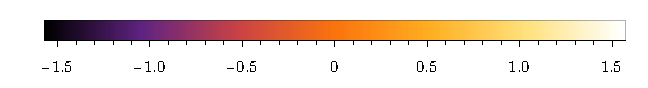
\includegraphics[scale=1.2]{../img/N=3_barA.pdf}
    \caption{Arctangens of the metric tensor for higher state manifolds. By  rows: $M_0$, $M_1$; $M_2$, $M_3$; $M_4$, $M_5$.}
    \label{fig:higherStateManifolds}    
\end{figure}


\begin{figure}[H]
    \centering
    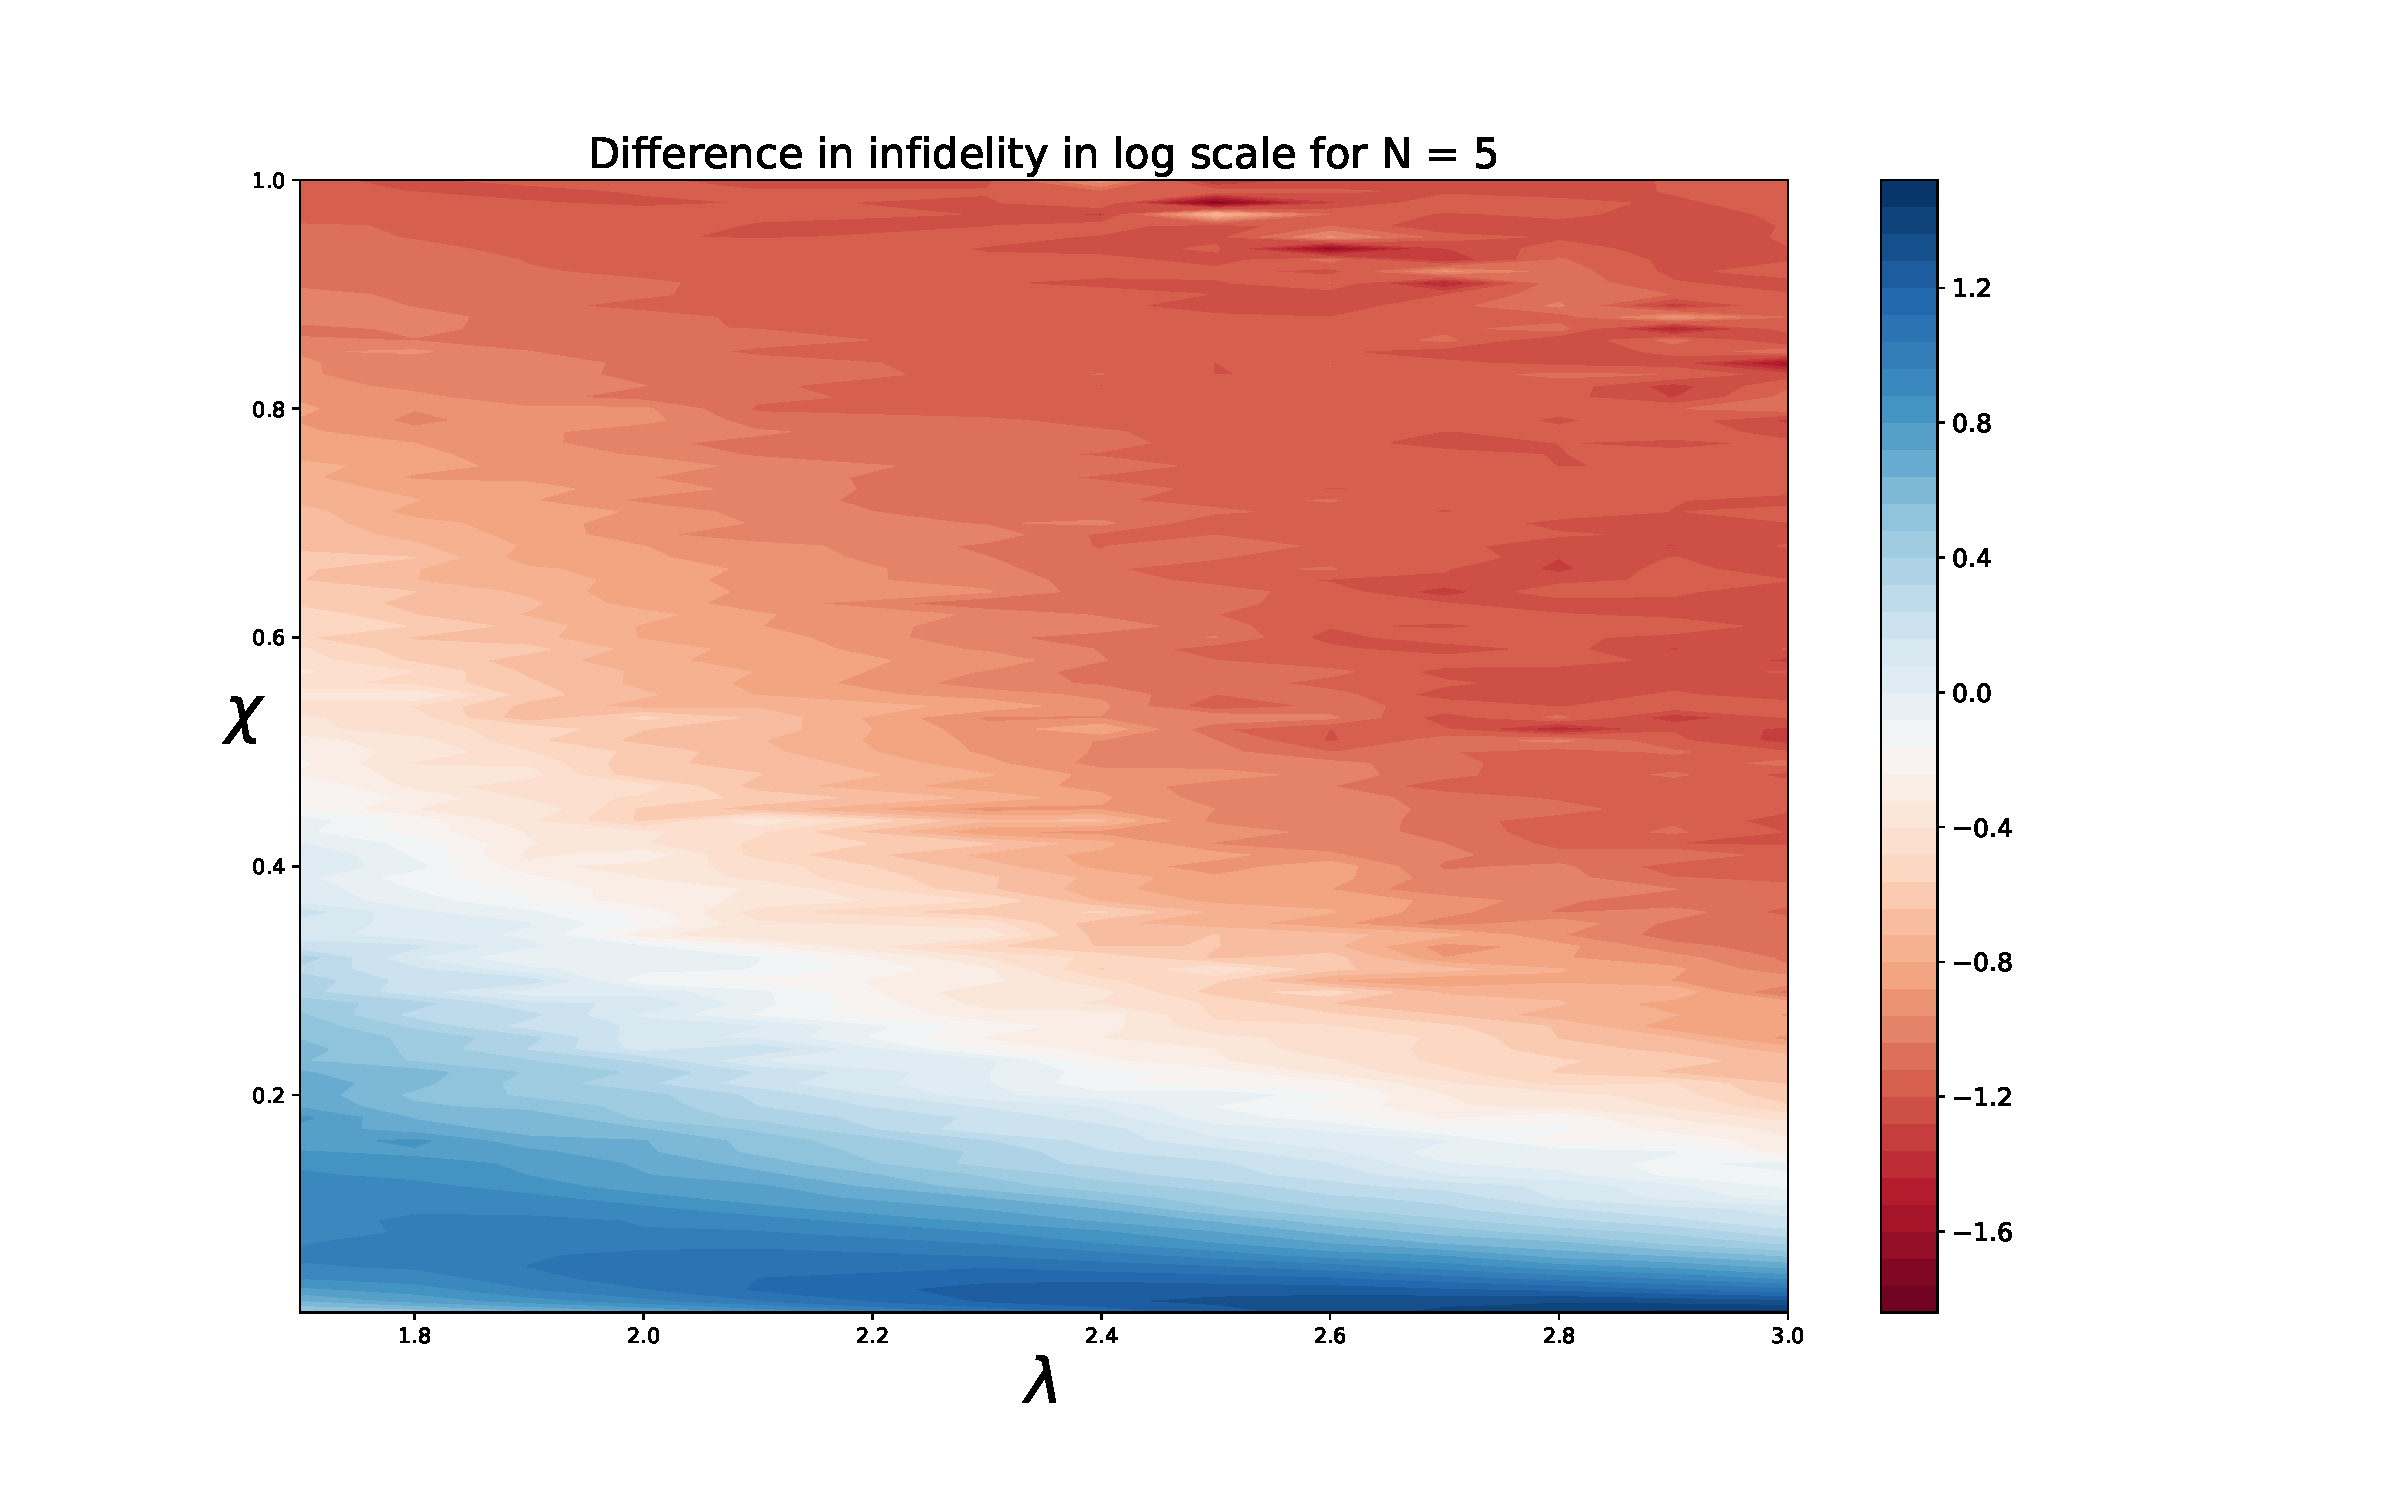
\includegraphics[width=1\textwidth]{../img/fidelity_lineVSgeodesic.pdf}
    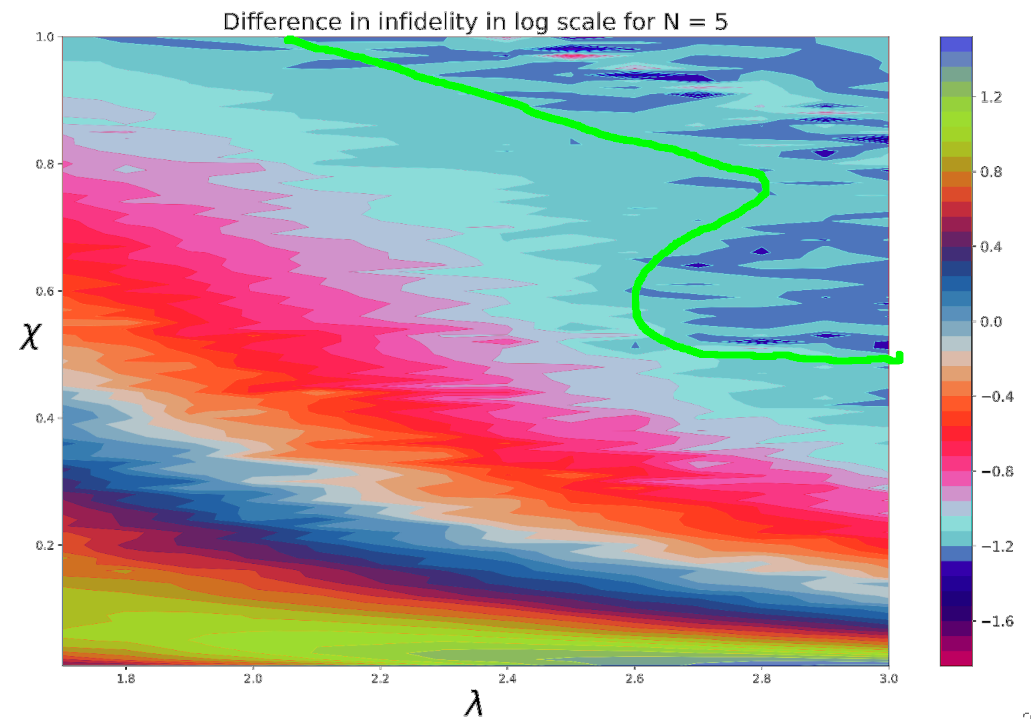
\includegraphics[width=0.8\textwidth]{../img/fidelity_geodesicVSline_fuckedupcolors.png}
    \caption{\textcolor{gray}{Infidelity difference between line and geodesic, above picture is original from Felipe, bottom one is edited in GIMP to see the difference more clearly.}}
    \label{fig:higherStateManifolds}    
\end{figure}





% \chapter{Two level system}
% Having a vector $\kpsi=(Z_0,Z_1)$, we can search for a geodesic on ground state manifold $\M_0$ by plugging metric tensor $g^{(0)}_{\mu\nu}$ from Eq. \ref{eq:metrictensork} into geodesic equation. This surely minimizes the distance on $\M_0$, but what meaning does it have on protocols inside the whole projective space $\PH$? 

% Let's once again consider Hamiltonian eigenbasis $\kpsi=Z_0\ket{0}+Z_1\ket{1}$, only here it depends on parameter $\llambda$. Using normalization we get
% \begin{equation}
%     \ket{\psi(\llambda)}=\cos \theta(\llambda) \ket{0(\llambda)}+e^{i\phi}\sin\theta \ket{1(\llambda)}
% \end{equation}
% and it's variation (omitting the dependence on $\llambda$ in every element)
% \begin{equation}
%     \delta\ket{\psi}=\delta Z_0 \ket{0}+ Z_0 \ket{\delta 0}-\delta Z_0 \ket{1}+ (1-Z_0) \ket{\delta 1}.
%     \label{eq:psiVariation}
% \end{equation}
% The projections $\braket{j|k+\delta k}$ are known from Eq. \ref{eq:braket_k,deltaj} and 
% \begin{equation}
%     \delta Z_0(\llambda)=Z_0(\llambda+\delta \llambda)-Z_0(\llambda)=\frac{\d Z_0}{\d \llambda^\mu}\d\llambda^\mu,
% \end{equation}
% where the last fraction is close to zero for drivings with low excitation rates. Distance of some transport in $\PH$ with free parameters $\llambda,Z_0$ is then according to Eq. \ref{eq:distanceInPH} (again imagine the $\llambda$ dependence in every element)
% \begin{equation}
%     \begin{split}
%         \d s^2\textcolor{gray}{(\llambda)} =& 1-|\braket{\delta \psi|\psi}|^2=1-\big|\underbrace{\braket{\delta 0|\overline{Z}_0 Z_0|0}}_{\propto \braket{\delta 0|0}=0}+\braket{\delta 0|\overline{Z}_0(1-Z_0)|1}\\
%         &+\braket{\delta 1| (1-\overline{Z}_0)Z_0|0}+\underbrace{\braket{\delta 1|(1-\overline{Z}_0)(1-Z_0)|1}}_{\propto \braket{\delta 1|1}=0}\big|^2\\
%         =&1-\Big| \overline{Z}_0(1-Z_0)\frac{\braket{0|\delta H|1}}{(E_1-E_0)^2} +\underbrace{(1-\overline{Z}_0)Z_0\frac{\braket{1|\delta H|0}}{(E_1-E_0)^2}}_{\text{c.c. of the first part}}\Big|^2\\
%         =&1-2\underbrace{\big|\overline{Z_0\textcolor{gray}{(\llambda)}}(1-Z_0\textcolor{gray}{(\llambda)})\big|^2}_{Z_0\text{-term}}\underbrace{\frac{\big|\braket{1\textcolor{gray}{(\llambda)}|\delta H\textcolor{gray}{(\llambda)}|0}\big|^2}{(E_1\textcolor{gray}{(\llambda)}-E_0\textcolor{gray}{(\llambda)})^2}}_{\llambda\text{-term}}.
%     \end{split}
% \end{equation}
% The $Z_0$-term can be minimized by setting $Z_0=0.5$ and the $\llambda$-term is smallest for a ground state manifold geodesic. This does not mean, that some combination of them is not better, than fulfilling those two conditions simultaneously. Plus the initial and final conditions need to have $Z_0=0.5$.












\chapter{The meaning of geodesics}


\section{Transport using quenches}
\label{sec:quenches}
Unifying the ground states $\ket{o(\llambda)}$ over all points $\llambda\in\R^n$ in the parameter space, we get the ground state manifold. Here the fidelity $f$ and distance $s$ are defined
\begin{equation}
    \d s^2 \equiv 1-f^2\equiv 1-\left|\braket{o(\bm\llambda+\delta\bm\llambda)|o(\bm\llambda)}\right|^2.
    \label{eq:distanceOnM0}
\end{equation}

The final fidelity of transport on $\M$ is then
\begin{equation}
    F=\iint g_{\mu\nu}\d\lambda^\mu\d\lambda^\nu = \int_{t_i}^{t_f}\underbrace{\int_{t_i}^\tau g_{\mu\nu}\der{\lambda^\mu}{t}\der{\lambda^\nu}{t} \d t}_{\mathcal{L}(\lambda^\mu,\dot\lambda^\mu,\tau)}\d \tau .
\end{equation}
Using Euler-Lagrange equations for time-independent $g_{\mu\nu}=g_{\mu\nu}(\lambda^\mu)$, leads to
\begin{equation}
    \int_{t_i}^{\tau}\left[g_{\mu\nu,\kappa}\dot\lambda^\mu\dot\lambda^\nu - \der{}{t}\left[g_{\mu\nu}\left(\delta^\mu_\kappa\dot\lambda^\nu+\dot\lambda^\mu\delta^\nu_\kappa\right)\right]\right]\d t=0,
\end{equation}
which needs to be zero for integration over any subset $(t_i,\tau)$. This can bne achieved for any path only it the integrand itself is zero, which happens if the geodesic equation holds.

The fidelity $f$ measures transition probability between two neighboring eigenstates of two different Hamiltonians. Those two states belong to the same Fibre space $\PH(\llambda)\times \R^n$ from which the coefficients $(\Z,\llambda)$ are taken. Because all $\PH(\llambda)$ are canonically isomorphic, there is no problem in parallel transport from one space to another, which is needed for braket\footnote{This procedure is done without thinking in the back part of our brains such, that we don't even think about it. That's how trivial it is.}.

The distance minimization runs into some interpretation problems. On one hand, minimalization of the distance is equivalent to maximalization of the sum of infinitezimal fidelities along the path (we say we \emph{maximize the fidelity along the path}). On the other hand we are using only ground states in every step of the transport, therefore defining the fidelity to be one. There are actually two ways out of this confusion. \emph{Perturbed adiabatic driving} and \emph{Transport using quenches}.


\subsubsection{Perturbed adiabatic driving}
It the first case, we imagine at every point of transport, that the fidelity is small enough, such that in eigenbasis and some small parameters $\delta_i\in \mathbb{C}$ we get
$$\ket{o(\llambda_i)}\equiv \begin{pmatrix}
    Z_0(\llambda_i)\\
    0\\
    \vdots \\
    0
\end{pmatrix} \overset{\text{transport }\d s}{\longrightarrow} \ket{o(\llambda_i+\delta \llambda)}\equiv\begin{pmatrix}
    Z_0(\llambda_i+\delta \llambda)\\
    0\\
    \vdots \\
    0
\end{pmatrix} +\underbrace{\begin{pmatrix}
    0\\
    \delta_1(\llambda_i+\delta \llambda)\\
    \vdots \\
    \delta_n(\llambda_i+\delta \llambda)
\end{pmatrix}}_{\mathbf{\Delta}(\llambda_i+\delta \llambda)}, $$
where the last term is neglected using 
$$\braket{\Delta(\llambda)|o(\llambda+\delta\llambda)}\approx 0.$$

This might have interesting implication for slow transports, or small distance transports. For example when some slow thermalization is considered during a transport.



\subsubsection{Transport using quenches}
If we imagine $\delta\llambda$ to be finite (not infinitely small, as the notation suggests), the \textbf{transport} means \textbf{doing a sequence of quenches and measuring the system after every quench}.


Some notion of the space of our Hamiltonian can be seen by quenching from $(\lambda_i;\chi_i)=(0;0)$ to $(\lambda;\chi)$, as can be seen in Figure \ref{fig:quenchFidelityFrom00}.

In Figure \ref{fig:equidistantPointsOnPath} are marked equidistant points, meaning $\int_a^b \d s=\text{const.}$ between every two neighboring points on curve. This means that if the system is measured periodically, the quenches jump smaller distances when closer to a singularity.

Decreasing time step $\Delta t$ has no effect on the relative fidelity of quenches during the evolution but has an effect on their magnitude. As one would expect from \emph{quantum Zeno effect}, when $\Delta t\rightarrow 0$, the transport becomes adiabatic, and the fidelity at any time will become 1. This can be observed in Figure \ref{fig:plotsFidelityQuenches}, such that the shape of the point-like paths looks similar in the columns, and their magnitude decreases.

The quantum Zeno effect for this case can be shown dirrectly by splitting the distance $s$ to $N$ equal pieces. The fidelity for $N$ splits will then be
\begin{equation}
    f(N)=(1-\Delta s)^N=\left(1-\left(\frac{s}{N}\right)^2\right)^N \;\;\overset{N\rightarrow\infty}{\longrightarrow}\;\; 1,
\end{equation}
meaning the consequent measurements will colapse the system to its instantenous eigenstate and the adiabatic condition for transport holds. 

Such measurements can be achieved by fast thermalization of the system. If the finite speed thermalization with $N=T/\tau$ for the mean time between two measurements $\tau$, we get
\begin{equation}
    \begin{split}
        \log f(N) &= N \log \left(1-\left(\frac{s}{N}\right)^2\right) = -\frac{s^2}{N}+o\left(\frac{s^4}{n^3}\right)\\
        f(N) &= \exp\left(-s^2\frac{\tau}{T}-\frac{s^4}{2 N^3}\dots\right) = \exp\left(-s^2\frac{\tau}{T}\right)\left(1+o\left(\frac{s^4}{N^3}\right)\right)
    \end{split}
\end{equation}


\begin{figure}[H]
    \centering
    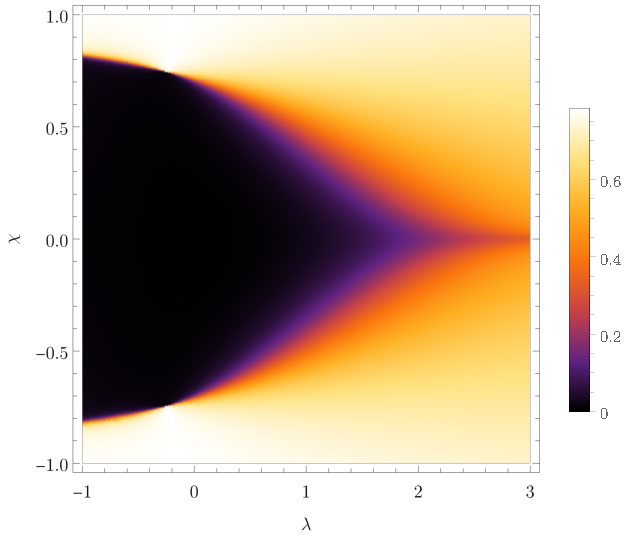
\includegraphics[scale=1.2]{../img/quenchFidelityFrom00.pdf}
    \caption{Arctangens of the fidelity of quenches from $(\lambda_i;\chi_i)=(0;0)$ to $(\lambda;\chi)$.}
    \label{fig:quenchFidelityFrom00}    
\end{figure}

\begin{figure}[H]
    \centering
    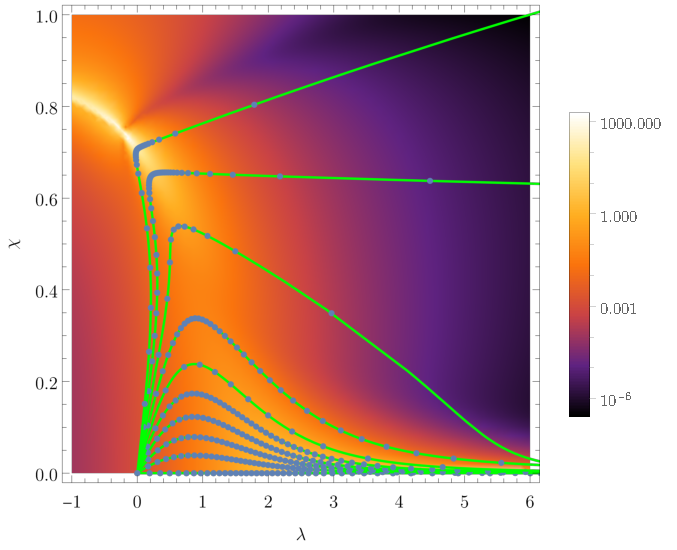
\includegraphics[scale=1.2]{../img/equidistantPointsOnPath.pdf}
    \caption{Equidistant points on geodesics of the ground state manifold.}
    \label{fig:equidistantPointsOnPath}    
\end{figure}

\begin{figure}[H]
    \centering
    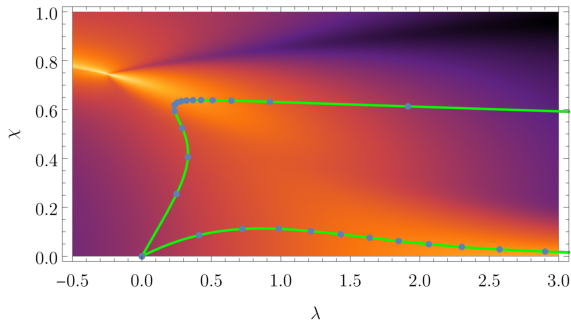
\includegraphics[scale=1.2]{../img/bg123.pdf}
    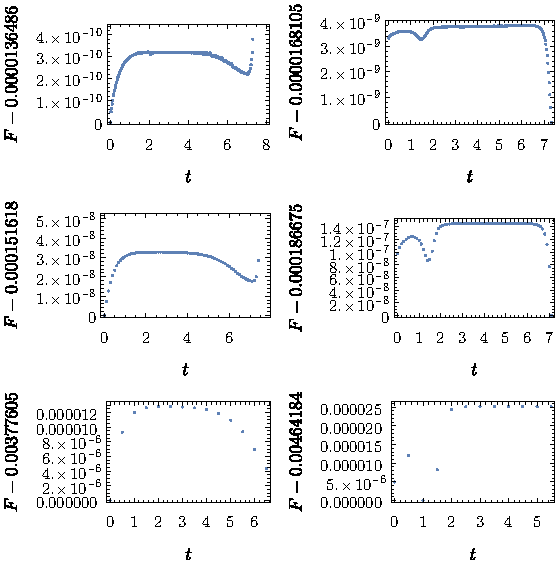
\includegraphics[scale=1.3]{../img/plotsFidelityQuenches.pdf}
    \caption{Fidelity for sequential quenches along geodesics (see green lines on top). Left (right) column corresponds to lower (upper) geodesic. Time steps from top are $\Delta t\in \{0.03,0.1,0.5\}$. Time difference between points in the plot on top is $\Delta t=0.5$.}
    \label{fig:plotsFidelityQuenches}    
\end{figure}



% \section{Higher state transition metric operator}


% When one assumes a function in a ground state at every point of transport, situation using quenches is reconstructed. During some general transport, in which a superposition of states is allowed, one also needs to minimize the flow of probability from higher states to even higher states and maximize the flow from higher states to lower ones. Let us try to construct a new metric tensor, which will count in those \emph{higher-state transition} effects.

% Imagine a driving
% \begin{align*}
%     \gamma:\R &\rightarrow \R^n \\
%     t &\mapsto \llambda\equiv (\lambda_1,\dots \lambda_n)
% \end{align*}
% This function translates the driving parameter $t$ to coordinates for Hamiltonian $\HH(\llambda)$. Assume the states
% \begin{equation}
%     \textcolor{teal}{\ket{\Psi(t)}=\sum_m a_m(t)\ket{m(t)}}
% \end{equation}
% for eigenstates $\ket{m(t)}$ of the Hamiltonian $\HH$. Now we can form a linear combination of effects on this wavefunction, where every excitation probability needs to be minimized and every deexcitation maximized. \textbf{Because $\partial_\mu \HH$ is a hermitian operator, the excitation and deexcitation will occur with the same probability. Plus if we assume the Fidelity to be $F>0.5$}, we can neglect the deexcitation probabilities and instead \textcolor{blue}{minimize only the excitations}, which can be done by introducing \emph{Higher state transition metric operator}, let's call it just the \emph{metric operator}\footnote{It's not a tensor, because it does not transform like a tensor. It depends on a path.}
% \begin{equation}
%     \begin{split}
%         G_{\mu\nu}^{\textcolor{teal}{\psi}(t)} =& \Re \sum\limits_{j=0}^n \textcolor{blue}{\sum_{m=j+1}^n}\textcolor{teal}{ a_m^*(t)a_m(t)}\frac{\textcolor{teal}{\bra{m(t)}}\pder{\HH(\gamma(t))}{\lambda^\mu}\ket{j}\bra{j}\pder{\HH(\gamma(t))}{\lambda^\nu}\textcolor{teal}{\ket{m(t)}}}{(E_{\textcolor{teal}{\psi}}(t)-E_j)^2}
%     \label{eq:metrictensorREdefinition}
%     \end{split}
% \end{equation}
% for the coefficient $E_\Psi(t)=\sum_{m>j} a_m(t) E_m$, which is a complex number has no meaning of energy. If  $a_0=1$ and $a_m=0$ for $m\in\{1,\dots,n\}$, we get the metric tensor $g^{(0)}_{\mu\nu}$ from Eq. \ref{eq:metrictensork}. The problem arises when those coefficients are nonzero, which makes the problem nonlinear in a sense

% \begin{figure}[H]
%     \centering
%     \begin{tikzpicture}[->,>=stealth',auto,node distance=2.5 cm,
%         thick,main node/.style={font=\sffamily\Large\bfseries}]
        
%         \node[main node] (1) {$a_m$};
%         \node[main node] (2) [right of=1] {$\psi(t)$};
%         \node[main node] (3) [right of=2] {$G_{\mu\nu}^{\psi(t)}$};
        
%         \path[every node/.style={font=\sffamily\small}]
%         (1) edge node [right] {} (2)
%         (2) edge node [right] {} (3)
%         (3) edge[bend right] node [left] {} (1);
%     \end{tikzpicture}
% \end{figure}

% To see how much Higher state manifolds influence the driving, we can compare some driving results with individual elements of the metric operator, see Figure \ref{fig:higherStateManifolds}. One such result which might support the hypothesis postulated in Eq. \ref{eq:metrictensork} is that geodesics will be much worse in the areas where the space is more curved in $M_1$. This also holds for $M_2$ etc., but the effect from $M_1$ will be strongest. For comparison see the metric tensor for higher state manifolds in Figure \ref{fig:higherStateManifolds}.

% \begin{figure}[H]
%     \centering
%     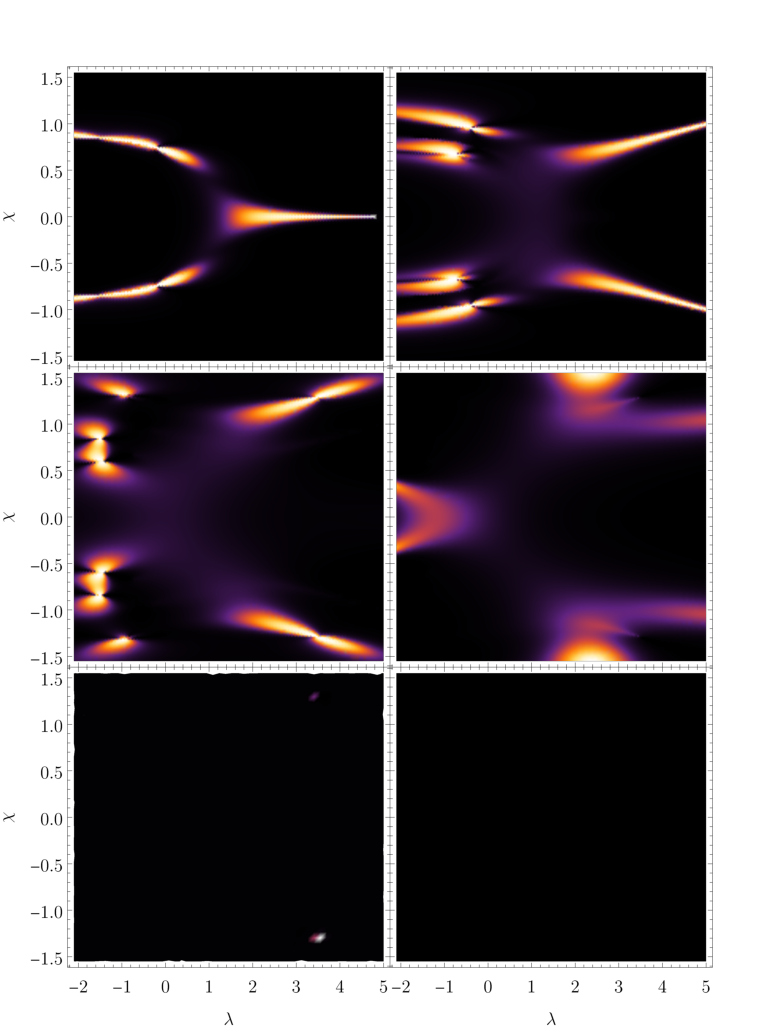
\includegraphics[scale=1.2]{../img/N=5_metricDeterminantElements.pdf}
%     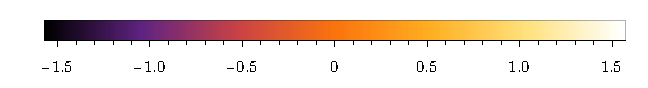
\includegraphics[scale=1.2]{../img/N=3_barA.pdf}
%     \caption{Arctangens of the elements of higher state manifolds. By rows using $j$ from the sum in eq. \ref{eq:metrictensorREdefinition}: $j=0$, $j=1$; $j=2$, $j=3$; $j=4$, $j=5$.}
%     \label{fig:metricDeterminantElements}    
% \end{figure}

% \begin{figure}[H]
%     \centering
%     \includegraphics[scale=1.2]{../img/N=5_metricDeterminants.pdf}
%     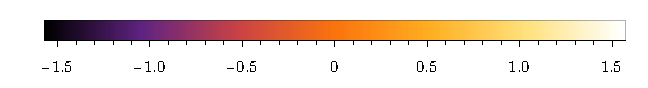
\includegraphics[scale=1.2]{../img/N=3_barA.pdf}
%     \caption{Arctangens of the metric tensor for higher state manifolds. By  rows: $M_0$, $M_1$; $M_2$, $M_3$; $M_4$, $M_5$.}
%     \label{fig:higherStateManifolds}    
% \end{figure}














% \chapter{Metric tensor of the higher state manifold}
% Definition of the k-state manifold is
% \begin{equation}
%     g_{\mu\nu}^{(k)} = \Re \sum_{j\neq k}\frac{\braket{k|\pder{\HH(\llambda)}{\lambda^\mu}|j}\braket{j|\pder{\HH(\llambda)}{\lambda^\nu}|k}}{(E_k-E_j)^2}.
%     \label{eq:metrictensork}
% \end{equation}
% One has to see it as a measure between the quantum states. The states are further away from each other when they are "more perpendicular" because the transition probability between the states is lower. The only difference here is that one state needs to be evolved using the derivative of Hamiltonian. From this goes that \emph{minimizing the distance on path} means \emph{going through the least excitation probability path}.

% When one assumes a pure ground state at every point of transport, the situation using quenches, see section \ref{sec:quenches}, is reconstructed. During some general transport, in which a superposition of states is allowed, one also needs to minimize the flow of probability from higher states to even higher states and maximize the flow from higher states to lower ones. Let us try to construct a new metric tensor, which will count in those \emph{higher-state transition} effects.

% \section{Higher state transition metric operator}
% Imagine a driving 
% \begin{align*}
%     \gamma:\R &\rightarrow \R^n \\
%     t &\mapsto \llambda\equiv (\lambda_1,\dots \lambda_n)
% \end{align*}
% This function translates the driving parameter $t$ to coordinates for Hamiltonian $\HH(\llambda)$. Assume the states
% \begin{equation}
%     \textcolor{purple}{\ket{\Psi(t)}=\sum_m a_m(t)\ket{m(t)}}
% \end{equation}
% for eigenstates $\ket{m(t)}$ of the Hamiltonian $\HH$. Now we can form a linear combination of effects on this wavefunction, where every excitation probability needs to be minimized and every deexcitation maximized. \textbf{Because $\partial_\mu \HH$ is a hermitian operator, the excitation and deexcitation will occur with the same probability. Plus if we assume the Fidelity to be $F>0.5$}, we can neglect the deexcitation probabilities and instead \textcolor{blue}{minimize only the excitations}, which can be done by introducing \emph{Higher state transition metric operator}, let's call it just the \emph{metric operator}\footnote{It's not a tensor, because it does not transform like a tensor. It depends on a path.}
% \begin{equation}
%     \begin{split}
%         G_{\mu\nu}^{\textcolor{purple}{\psi}(t)} =& \Re \sum\limits_{j=0}^n \textcolor{blue}{\sum_{m=j+1}^n}\textcolor{purple}{ a_m^*(t)a_m(t)}\frac{\textcolor{purple}{\bra{m(t)}}\pder{\HH(\gamma(t))}{\lambda^\mu}\ket{j}\bra{j}\pder{\HH(\gamma(t))}{\lambda^\nu}\textcolor{purple}{\ket{m(t)}}}{(E_{\textcolor{purple}{\psi}}(t)-E_j)^2}
%     \label{eq:metrictensorREdefinition}
%     \end{split}
% \end{equation}
% for the coefficient $E_\Psi(t)=\sum_{m>j} a_m(t) E_m$, which is a complex number has no meaning of energy. If  $a_0=1$ and $a_m=0$ for $m\in\{1,\dots,n\}$, we get the metric tensor $g^{(0)}_{\mu\nu}$ from Eq. \ref{eq:metrictensork}. The problem arises when those coefficients are nonzero, which makes the problem nonlinear in a sense

% \begin{figure}[H]
%     \centering
%     \begin{tikzpicture}[->,>=stealth',auto,node distance=2.5 cm,
%         thick,main node/.style={font=\sffamily\Large\bfseries}]
        
%         \node[main node] (1) {$a_m$};
%         \node[main node] (2) [right of=1] {$\psi(t)$};
%         \node[main node] (3) [right of=2] {$G_{\mu\nu}^{\psi(t)}$};
        
%         \path[every node/.style={font=\sffamily\small}]
%         (1) edge node [right] {} (2)
%         (2) edge node [right] {} (3)
%         (3) edge[bend right] node [left] {} (1);
%     \end{tikzpicture}
% \end{figure}

% To see how much Higher state manifolds influence the driving, we can compare some driving results with individual elements of the metric operator, see Figure \ref{fig:higherStateManifolds}. One such result which might support the hypothesis postulated in Eq. \ref{eq:metrictensork} is that geodesics will be much worse in the areas where the space is more curved in $M_1$. This also holds for $M_2$ etc., but the effect from $M_1$ will be strongest. For comparison see the metric tensor for higher state manifolds in Figure \ref{fig:higherStateManifolds}.

% \begin{figure}[H]
%     \centering
%     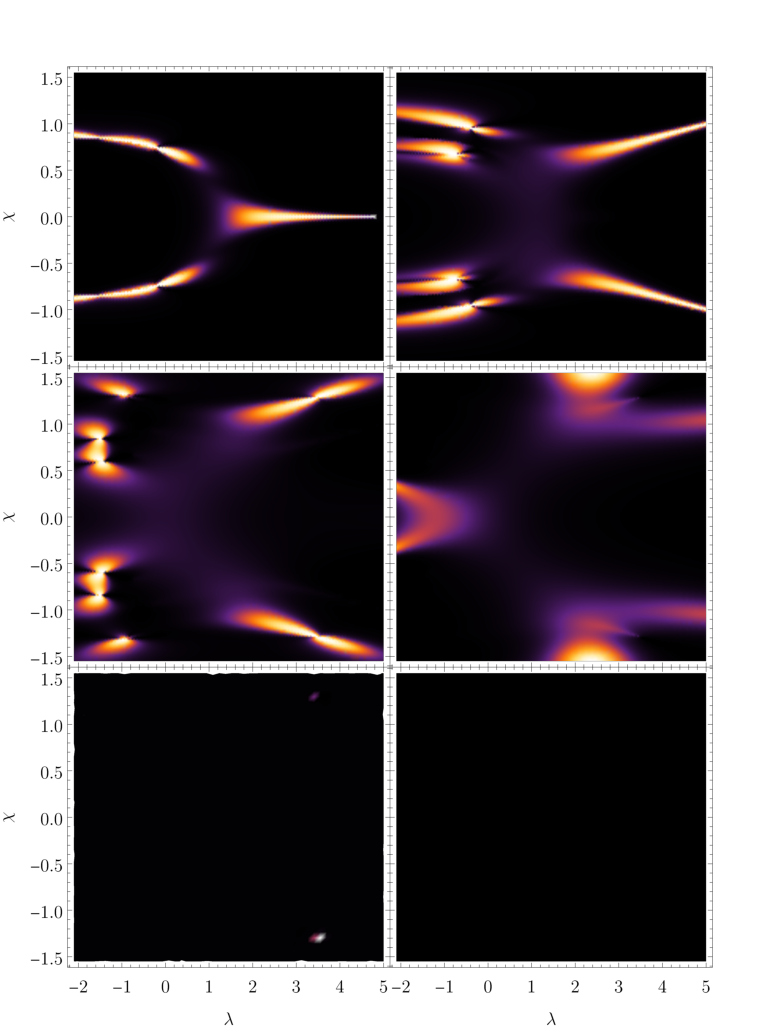
\includegraphics[scale=1.2]{../img/N=5_metricDeterminantElements.pdf}
%     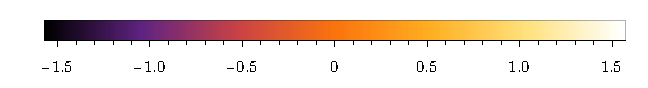
\includegraphics[scale=1.2]{../img/N=3_barA.pdf}
%     \caption{Arctangens of the elements of higher state manifolds. By rows using $j$ from the sum in eq. \ref{eq:metrictensorREdefinition}: $j=0$, $j=1$; $j=2$, $j=3$; $j=4$, $j=5$.}
%     \label{fig:metricDeterminantElements}    
% \end{figure}

% \begin{figure}[H]
%     \centering
%     \includegraphics[scale=1.2]{../img/N=5_metricDeterminants.pdf}
%     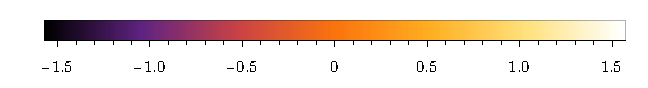
\includegraphics[scale=1.2]{../img/N=3_barA.pdf}
%     \caption{Arctangens of the metric tensor for higher state manifolds. By  rows: $M_0$, $M_1$; $M_2$, $M_3$; $M_4$, $M_5$.}
%     \label{fig:higherStateManifolds}    
% \end{figure}

